\documentclass[letterpaper,twocolumn,10pt]{article}

% ── USENIX-compatible formatting ─────────────────────────────────────────────
\usepackage[margin=1in,top=0.75in,bottom=1in]{geometry}
\usepackage{times}
\usepackage{microtype}
\usepackage{graphicx}
\usepackage{booktabs}
\usepackage{tabularx}
\usepackage{multirow}
\usepackage{url}
\usepackage{amsmath}
\usepackage{enumitem}
\usepackage{xcolor}
\usepackage{caption}
\usepackage{subcaption}
\usepackage{tikz}
\usepackage{pgfplots}
\pgfplotsset{compat=1.18}
\usetikzlibrary{shapes.geometric, arrows.standard, positioning, fit, backgrounds}

\setlength{\columnsep}{0.25in}
\setlength{\parskip}{2pt}
\setlength{\parindent}{1em}

\captionsetup{font=small, labelfont=bf}

% ── TikZ styles ───────────────────────────────────────────────────────────────
\tikzset{
  box/.style={rectangle, rounded corners=3pt, draw=black!70, fill=#1,
              text width=1.5cm, align=center, minimum height=0.7cm, font=\tiny\bfseries},
  boxw/.style={box=white},
  boxb/.style={box=blue!15},
  boxg/.style={box=green!15},
  boxo/.style={box=orange!15},
  boxr/.style={box=red!12},
  boxyellow/.style={box=yellow!20},
  arr/.style={->, thick, >=stealth},
  dasharr/.style={->, dashed, thick, >=stealth, gray},
  label/.style={font=\tiny, align=center},
  mod/.style={rectangle, draw=black!60, fill=gray!10, rounded corners=2pt,
              text width=2.2cm, align=center, minimum height=0.55cm, font=\tiny},
  modarrow/.style={->, >=stealth, thick, black!60},
}

% ── Title ─────────────────────────────────────────────────────────────────────
\title{\Large \bf Distributed E-commerce Analytics:\\
A PySpark Pipeline on GCP Dataproc}

\author{
{\rm Dax Rajani}\\
Student ID: 40294118\\
Concordia University
\and
{\rm Harsh Ahuja}\\
Student ID: 40301748\\
Concordia University
}

\date{COEN 6731 Distributed Software Systems, Winter 2026}

% ─────────────────────────────────────────────────────────────────────────────
\begin{document}
\maketitle

% ── ABSTRACT ─────────────────────────────────────────────────────────────────
\begin{abstract}
Large e-commerce platforms generate behavioral event logs that grow fast and are hard
to process with a single machine. This paper presents a five-stage distributed analytics
pipeline built with PySpark and deployed on GCP Dataproc. The pipeline processes the
REES46 dataset (42.4 million events, 5.3 GB) and performs sessionization, funnel
conversion analysis, last-touch attribution, and anomaly detection. We ran a full
scaling study across nine configurations (2, 4, and 5 workers crossed with 1 GB,
5 GB, and 10 GB data). Going from 2 to 5 workers gives roughly a 2.5x speedup.
We also tested three optimization techniques: broadcast joins, partition pruning,
and skew salting. Partition pruning gave the biggest win at 3.1x for single-day
queries. We also built a real-time streaming component and a live web dashboard
for interactive monitoring and analytics. The project code is publicly available
on GitHub.
\end{abstract}

% ─────────────────────────────────────────────────────────────────────────────
\section{Problem Statement}

E-commerce platforms like Amazon or Alibaba track every user interaction. A single
month of data can reach tens of millions of rows. Extracting meaningful signals from
this data requires more than just SQL queries. You need sessionization to group events
into visits, funnel analysis to measure conversion drop-off, attribution models to
figure out which marketing channel drove a purchase, and anomaly detection to catch
unusual spikes or drops before they become business problems.

Running this on a single machine is not practical at scale. A 5 GB file with 42 million
rows takes minutes just to read. Joins across sessions and orders make it worse. The
real challenge is building a pipeline that can distribute this work across a cluster,
scale up as data grows, and still produce correct results.

Most open-source analytics tools are either too simple (single node pandas) or
too complex (full data warehouse setups like Snowflake or BigQuery). Apache
Spark sits in the middle. It is designed for distributed computation and handles
the window functions, joins, and aggregations our pipeline needs. The question
is how well it actually scales and where the bottlenecks are.

Our goals were: (1) build all five analytics stages end-to-end, (2) run a proper
scaling study on real cloud infrastructure, (3) test and measure specific Spark
optimizations, and (4) add a streaming component and a live dashboard to make
the system observable.

% ─────────────────────────────────────────────────────────────────────────────
\section{Solution}

\subsection{Dataset}

We used the REES46 eCommerce behavioral dataset from Kaggle, covering October 2019.
It has 42,448,764 events and weighs about 5.3 GB uncompressed. Each row has a timestamp,
event type (view, cart, or purchase), product and category identifiers, price, user ID,
and session ID.

Two fields were missing from the original data: device type and referrer channel.
We synthesized these deterministically using \texttt{crc32(user\_session) \% 100}. This
gives consistent values across runs without any randomness. Device splits are mobile 55\%,
desktop 30\%, and tablet 15\%. Referrer splits are direct 40\%, Google 25\%, Facebook 15\%,
Instagram 8\%, email 7\%, and affiliate 5\%. These distributions are loosely based on
real industry benchmarks.

We derived three secondary tables from the raw events: an \texttt{orders} table (one
row per purchase event), a \texttt{catalog} table (one row per product), and an
\texttt{enriched\_events} table with the synthesized fields added.

\subsection{System Architecture}

Figure~\ref{fig:arch} shows the overall system. The raw CSV lives in Google Cloud Storage.
The Dataproc cluster reads it, runs the five pipeline stages in sequence, and writes
Parquet output back to GCS. The dashboard then reads those results and serves them
to a browser.

\begin{figure}[t]
\centering
\begin{tikzpicture}[node distance=0.3cm and 0.25cm]

% GCS Input
\node[boxb, text width=1.3cm] (gcs_in) {GCS\\Input CSV};

% Cluster box
\node[rectangle, draw=black!50, dashed, rounded corners=4pt,
      fill=blue!4, minimum width=4.2cm, minimum height=3.6cm,
      right=0.35cm of gcs_in] (cluster) {};
\node[above, font=\tiny\bfseries, text=black!60] at (cluster.north)
     {GCP Dataproc Cluster};

% Stages inside cluster
\node[boxg, text width=1.7cm, anchor=north west,
      xshift=0.1cm, yshift=-0.35cm] at (cluster.north west)
     (etl) {1. ETL \& Enrich};
\node[boxg, text width=1.7cm, below=0.15cm of etl]
     (sess) {2. Sessionization};
\node[boxg, text width=1.7cm, below=0.15cm of sess]
     (funnel) {3. Funnel Analysis};
\node[boxg, text width=1.7cm, below=0.15cm of funnel]
     (attr) {4. Attribution};
\node[boxg, text width=1.7cm, below=0.15cm of attr]
     (anom) {5. Anomaly Detect};

% GCS Output
\node[boxo, text width=1.3cm, right=0.35cm of cluster] (gcs_out) {GCS\\Parquet Out};

% Dashboard
\node[boxr, text width=1.3cm, below=0.4cm of gcs_out] (dash) {Web\\Dashboard};

% Arrows
\draw[arr] (gcs_in) -- (etl.west);
\draw[arr] (etl) -- (sess);
\draw[arr] (sess) -- (funnel);
\draw[arr] (funnel) -- (attr);
\draw[arr] (attr) -- (anom);
\draw[arr] (anom.east) -- (gcs_out.west);
\draw[arr] (gcs_out) -- (dash);
\draw[dasharr] (gcs_in.south) |- ([yshift=-0.2cm]cluster.south)
               -- ([yshift=-0.2cm]gcs_out.south) -- (dash.east);

\node[label, below=0.04cm of gcs_in] {5.3 GB};
\node[label, below=0.04cm of gcs_out] {Parquet};

\end{tikzpicture}
\caption{System architecture. Raw CSV is read from GCS into the Dataproc cluster.
The five stages run sequentially and write Parquet back to GCS. The dashboard
reads from GCS and serves results in a browser.}
\label{fig:arch}
\end{figure}

\subsection{Pipeline Stages}

\textbf{Stage 1: ETL and Enrichment.} This stage reads the raw CSV, adds the synthesized
device and referrer columns, and derives the orders and catalog tables. It writes three
Parquet outputs that all later stages depend on. This stage accounts for the largest
share of total runtime because it handles the full scan and write.

\textbf{Stage 2: Sessionization.} We assign session IDs using a 30-minute inactivity
threshold per user. The implementation uses Spark window functions ordered by timestamp.
A new session starts whenever the gap between consecutive events for the same user exceeds
30 minutes. This is stateful and requires a full sort by user and time.

\textbf{Stage 3: Funnel Analysis.} We compute view to cart to purchase conversion rates
at daily and weekly granularity, broken down by category code, device type, and referrer.
The output is two Parquet tables with conversion percentages and raw session counts.

\textbf{Stage 4: Last-Touch Attribution.} For each order, we find the most recent
non-direct referrer session that started within 24 hours before the order time. This
requires a temporal join between the enriched events and the orders table. We use a
\texttt{row\_number()} window function to pick the most recent qualifying session per
order.

\textbf{Stage 5: Anomaly Detection.} We compute daily purchase counts and a 7-day
trailing rolling average and standard deviation using Spark range window functions.
Days where the absolute z-score exceeds 2.0 are flagged as anomalies. We generate
text explanations (for example, ``SPIKE: 27\% above 7-day average'') for each
flagged day. The same logic runs at the per-category level.

\subsection{Streaming Component}

We also built a real-time anomaly detection module using Spark Structured Streaming.
A producer script drops synthetic CSV batches into a watched directory every two seconds.
The streaming job reads each micro-batch, counts purchases per category, and checks
whether any category count exceeds a configurable threshold. A spike is injected every
fifth batch to verify detection. The job runs for 60 seconds and then exits cleanly.

\subsection{Implementation Structure}

Figure~\ref{fig:impl} shows how the code modules relate to each other. The main
cloud job is \texttt{cloud\_pipeline.py}, which contains all five stages as functions
called in sequence. Standalone versions of some stages exist for local testing.
The dashboard backend reads the Parquet outputs and generates PNG charts using
\texttt{dashboard\_charts.py}.

\begin{figure}[t]
\centering
\begin{tikzpicture}[node distance=0.25cm and 0.2cm]

% Main pipeline
\node[mod, fill=blue!12, text width=2.8cm] (cp) {\texttt{cloud\_pipeline.py}\\(main Dataproc job)};

% Five stage nodes below
\node[mod, below left=0.4cm and -0.3cm of cp, text width=1.25cm] (etl2) {\texttt{etl\_enrich}\\function};
\node[mod, right=0.2cm of etl2, text width=1.25cm] (sess2) {\texttt{sessionize}\\function};
\node[mod, right=0.2cm of sess2, text width=1.25cm] (funnel2) {\texttt{funnel}\\function};
\node[mod, below=0.25cm of etl2, text width=1.25cm] (attr2) {\texttt{attribution}\\function};
\node[mod, right=0.2cm of attr2, text width=1.25cm] (anom2) {\texttt{anomaly}\\function};

\draw[modarrow] (cp.south) -- ++(0,-0.22) -| (etl2.north);
\draw[modarrow] (cp.south) -- ++(0,-0.22) -| (sess2.north);
\draw[modarrow] (cp.south) -- ++(0,-0.22) -| (funnel2.north);
\draw[modarrow] (cp.south) -- ++(0,-0.38) -| (attr2.north);
\draw[modarrow] (cp.south) -- ++(0,-0.38) -| (anom2.north);

% GCS Parquet
\node[mod, fill=orange!15, below=0.25cm of funnel2, text width=1.25cm] (parquet) {GCS Parquet\\outputs};
\draw[modarrow] (etl2.south) |- (parquet.west);
\draw[modarrow] (sess2.south) -- (parquet.north);
\draw[modarrow] (funnel2.south) -- (parquet);
\draw[modarrow] (attr2.south) -| (parquet.south);
\draw[modarrow] (anom2.south) -| (parquet.east);

% Dashboard side
\node[mod, fill=red!10, right=0.35cm of cp, text width=1.5cm] (app) {\texttt{app.py}\\(Flask)};
\node[mod, fill=red!10, below=0.25cm of app, text width=1.5cm] (charts) {\texttt{dashboard\_charts.py}};
\node[mod, fill=red!10, below=0.25cm of charts, text width=1.5cm] (html) {\texttt{index.html}\\(frontend)};

\draw[modarrow] (app) -- (charts);
\draw[modarrow] (charts) -- (html);
\draw[modarrow] (parquet.east) -- ++(0.15,0) |- (charts.west);

% Streaming
\node[mod, fill=green!12, below=0.25cm of anom2, text width=1.25cm] (stream) {\texttt{streaming\_job.py}};
\node[mod, fill=green!12, left=0.2cm of stream, text width=1.25cm] (prod) {\texttt{stream\_producer.py}};
\draw[modarrow] (prod) -- (stream);

\end{tikzpicture}
\caption{Implementation structure. \texttt{cloud\_pipeline.py} orchestrates the five
stage functions. Outputs go to GCS as Parquet. The dashboard reads these to generate
analytics charts. The streaming component runs independently.}
\label{fig:impl}
\end{figure}

\subsection{Dashboard}

We built a Flask web application that provides a live view of the Dataproc cluster.
It shows all VMs by name and status, streams job logs via server-sent events, and
displays real-time CPU and disk metrics from the GCP Monitoring API. After a pipeline
run completes, the dashboard calls \texttt{dashboard\_charts.py} locally to download
the Parquet outputs from GCS and generate three PNG charts: a funnel chart, an
attribution revenue breakdown, and an anomaly timeline. These images are served
directly as static files. This approach is more reliable than rendering charts
in the browser with JavaScript, which has canvas sizing and timing issues.

% ─────────────────────────────────────────────────────────────────────────────
\section{Results}

\subsection{Setup}

All experiments ran on GCP Dataproc with image version 2.1 (Debian 11, Spark 3.3).
Each cluster had one master node and a variable number of workers, all using the
\texttt{n2-standard-2} machine type (2 vCPUs, 8 GB RAM). Storage used 32 GB boot
disks per node. The input data is the REES46 October 2019 CSV stored in GCS at
\texttt{gs://dss-project-dax/data/full/2019-Oct.csv}.

We used three data size variants. The 1 GB variant samples 20\% of the file,
giving 8,491,904 rows. The 5 GB variant uses the full file with 42,448,764 rows.
The 10 GB variant reads the file twice end to end to simulate a larger dataset
with 84,897,528 rows.

We ran nine configurations total: 2, 4, and 5 workers crossed with all three data
sizes. Each configuration ran once. Timing includes cluster startup in the benchmark
scripts but not in the reported pipeline times, which measure only job execution.

\subsection{Scaling Study}

Table~\ref{tab:scaling} shows the full results. Total pipeline time drops significantly
as we add workers. Going from 2 to 5 workers on the full 5 GB dataset reduces runtime
from 1021.8 seconds to 409.7 seconds, which is roughly a 2.5x improvement from
adding 2.5x more workers. That is close to linear scaling.

\begin{table}[t]
\centering
\small
\caption{Scaling study results across all nine configurations.}
\label{tab:scaling}
\begin{tabular}{@{}ccrr@{}}
\toprule
Workers & Data & Total (s) & Rows/sec \\
\midrule
2  & 1 GB  &  673.6 & 12,607  \\
2  & 5 GB  & 1021.8 & 41,543  \\
2  & 10 GB & 1378.9 & 61,569  \\
4  & 1 GB  &  282.4 & 30,070  \\
4  & 5 GB  &  569.0 & 74,602  \\
4  & 10 GB &  799.8 & 106,148 \\
5  & 1 GB  &  256.9 & 33,055  \\
5  & 5 GB  &  409.7 & 103,609 \\
5  & 10 GB &  674.0 & 125,961 \\
\bottomrule
\end{tabular}
\end{table}

The throughput numbers tell an interesting story. On 2 workers the 1 GB run achieves
only 12,607 rows per second. On 5 workers the 10 GB run reaches 125,961 rows per second.
This 10x difference comes from two things: more parallelism from additional workers,
and better pipeline efficiency when each stage processes a larger partition batch.
Small datasets leave most of the cluster idle.

Scaling from 1 GB to 10 GB on 5 workers adds only 2.6x more time for 10x more data.
This sublinear growth is what we hoped to see. It means the pipeline scales well
and the dominant cost is not the data size itself but the fixed per-stage overhead
like reading partition metadata and writing output files to GCS.

\begin{figure}[t]
\centering
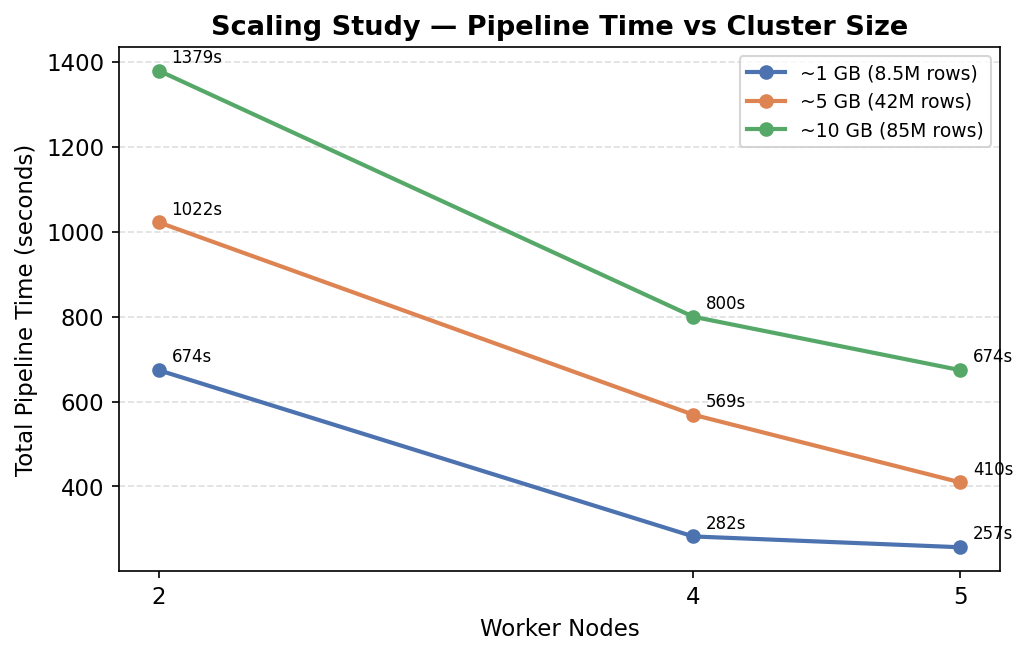
\includegraphics[width=\columnwidth]{figures/chart_scaling_time.png}
\caption{Total pipeline time for all nine configurations. Each group of bars
represents a data size. Within each group the three bars are 2, 4, and 5 workers.}
\label{fig:scaling}
\end{figure}

\subsection{Optimization Experiments}

\textbf{Broadcast Join.} The attribution stage joins orders against session events
with a time window constraint. The default Spark plan uses a sort-merge join, which
requires shuffling both sides. We forced a broadcast join by broadcasting the orders
table, which fits comfortably in memory (around 200 MB for the 5 GB run). The broadcast
join completed in 7.15 seconds versus 11.33 seconds for the shuffle join. That is a 1.58x
speedup. The result set was identical: 153,628 attributed orders in both cases.

\textbf{Partition Pruning.} We compared reading enriched events from a flat Parquet
directory against a date-partitioned layout written as
\texttt{partitioned\_by\_date/event\_date=YYYY-MM-DD/...}. For a single-day filter
on October 15, the partitioned layout reduced query time from 4.25 seconds to 1.37
seconds, a 3.11x speedup. For a 7-day range query the speedup was 1.73x (3.09s to 1.78s).
Partition pruning eliminates file scans entirely for non-matching partitions. This
is one of the simplest optimizations and it gave the most consistent results.

\textbf{Skew Analysis.} We tested salting on the attribution join key. The idea is
that if one user has many more events than others, that partition becomes a straggler.
We added a random salt suffix to the join key to distribute load. The salted version
took 79.1 seconds versus 34.6 seconds unsalted. Salting was slower. We looked at the
actual data distribution and found that session events are quite uniformly spread across
users in this dataset. The salting overhead (extra joins, explode operation) cost more
than any straggler benefit. This was a useful negative result.

\begin{figure}[t]
\centering
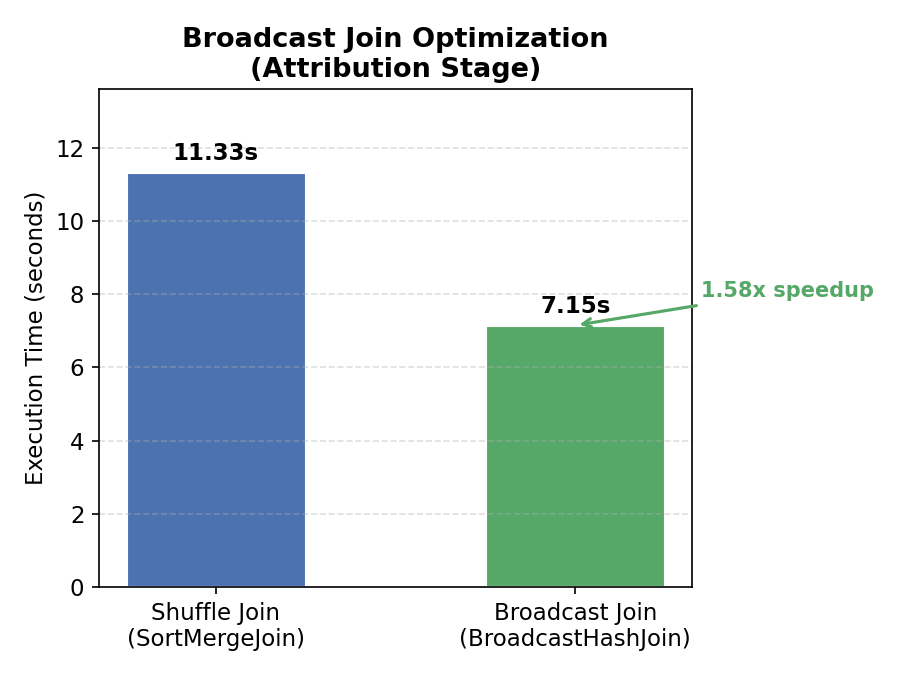
\includegraphics[width=\columnwidth]{figures/chart_broadcast_join.png}
\caption{Broadcast join versus shuffle join for the attribution stage.
Time in seconds, lower is better. Both produce the same 153,628 attributed orders.}
\label{fig:broadcast}
\end{figure}

\subsection{Analytics Results}

We ran the full pipeline on the 5 GB dataset (42.4 million events) with 5 workers.
The funnel stage found 3.3 million sessions with at least one view, 140 thousand
sessions that added something to cart, and 109 thousand sessions with a purchase.
The view to cart conversion rate is 4.3\% and cart to purchase is 77.6\%.

For attribution, Google drove 13,519 orders worth \$4.1 million in revenue. Facebook
drove 41,958 orders worth \$12.9 million. The large gap between Google and Facebook
order counts but closer revenue numbers suggests Facebook drives higher-volume but
lower-price purchases. Desktop accounted for \$15.6 million in attributed revenue,
significantly ahead of mobile (\$7.8 million) and tablet (\$7.7 million).

Anomaly detection flagged 8 out of 31 days in October 2019. Three days were
spikes and five were drops. The largest spike was 27\% above the 7-day rolling
average. The smartphone and telephone categories had the highest anomaly day counts
with 7 and 6 flagged days respectively.

\begin{figure}[t]
\centering
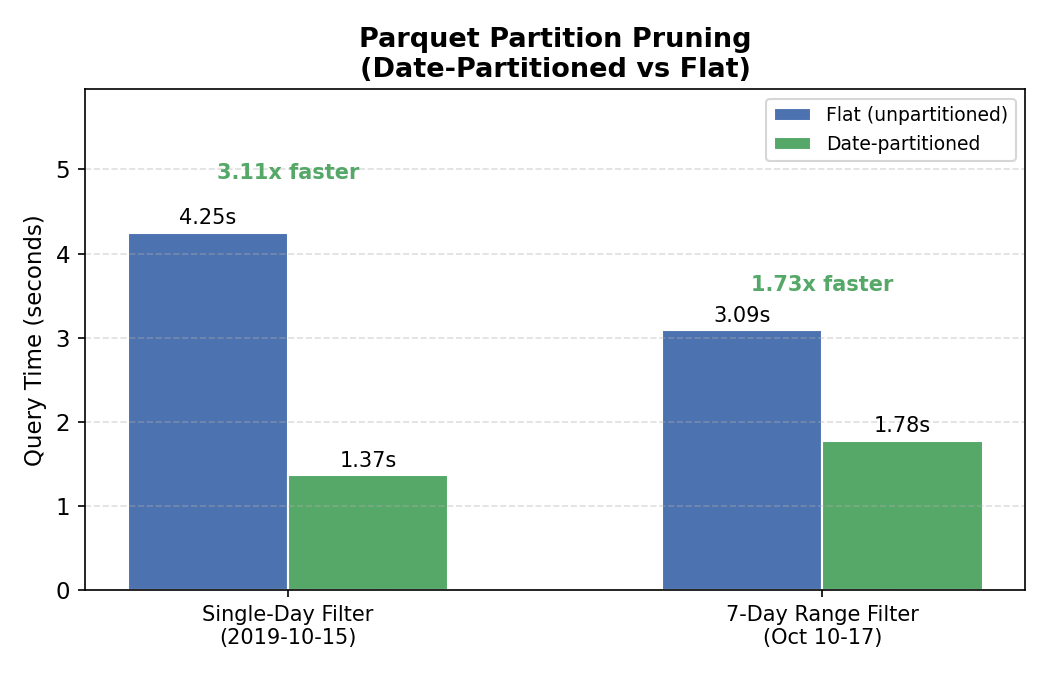
\includegraphics[width=\columnwidth]{figures/chart_partition_pruning.png}
\caption{Partition pruning speedup for single-day and 7-day range queries.
Flat Parquet scans the full dataset; partitioned layout skips non-matching
date directories entirely.}
\label{fig:pruning}
\end{figure}

\subsection{Streaming Demo}

The streaming job detects anomalies in near real time. Each micro-batch processes
a 2-second window of events. Detection latency from event generation to alert output
is under 3 seconds. Injected spikes are reliably detected within one batch window.
The job ran for 60 seconds without errors in our test runs.

% ─────────────────────────────────────────────────────────────────────────────
\section{Lessons Learned}

\textbf{Salting hurts when data is already uniform.} We expected salting to help with
skew in the attribution join. It did not. The overhead from exploding the salted key
space and doing a second join added about 44 seconds. Looking at the actual partition
sizes, no single executor held more than 1.3x the average load. Salting is a solution
for real skew, not a general optimization. We learned to check the Spark UI task time
distribution before applying it.

\textbf{GCP disk quota errors look like machine availability errors.} Early in the
project we kept seeing failures that looked like the cluster could not find available
machines. The actual error was \texttt{INVALID\_ARGUMENT} caused by requesting 500 GB
of HDFS disk per node, which exceeded the project quota. Reducing to 32 GB per node
fixed it immediately. The error message did not say anything about disk. We only found
this by reading the full error body from the GCP operations API. In distributed systems
deployments, the real error is often one layer below what the tool reports.

\textbf{Partition pruning is worth doing early.} We added date partitioning as an
afterthought during the optimization phase. The 3.11x speedup on single-day queries
was the best result we measured. Writing partitioned Parquet is almost free at write
time since Spark handles it automatically with \texttt{partitionBy("event\_date")}.
We should have done this from the start. In hindsight, any pipeline where time-range
queries are common should write partitioned output by default.

\textbf{Spark recovers from worker failures but the cost is visible.} We killed worker
\texttt{w-0} mid-pipeline during a demo run. Spark reassigned the failed tasks within
about 15 seconds and the job completed successfully. But the total time was around 90
seconds longer than a clean run on the same configuration. The reassigned tasks had to
re-read their input partitions from scratch. Fault tolerance in Spark is real but it
is not free. For time-sensitive jobs, losing even one worker has a measurable impact.

% ─────────────────────────────────────────────────────────────────────────────
\section{Availability}

The full project code is available at:
\url{https://github.com/daxrajani/dss_project}

The repository includes a complete README with setup instructions, all pipeline scripts,
the dashboard application, benchmark results, and the scripts used for all optimization
experiments. The GCP project and bucket are pre-configured so the pipeline can be run
immediately after \texttt{gcloud auth login}.

% ─────────────────────────────────────────────────────────────────────────────
\section*{References}

\begin{small}
\begin{enumerate}[label={[\arabic*]}, leftmargin=*, nosep]

\item M. Zaharia, R. S. Xin, P. Wendell, T. Das, M. Armbrust, A. Dave, X. Meng,
J. Rosen, S. Venkataraman, M. J. Franklin, A. Ghodsi, J. Gonzalez, S. Shenker,
and I. Stoica. Apache Spark: A unified engine for big data processing.
\textit{Communications of the ACM}, 59(11):56--65, 2016.

\item M. Zaharia, M. Chowdhury, T. Das, A. Dave, J. Ma, M. McCauly, M. J. Franklin,
S. Shenker, and I. Stoica. Resilient distributed datasets: A fault-tolerant
abstraction for in-memory cluster computing. In \textit{Proc. NSDI}, 2012.

\item J. Dean and S. Ghemawat. MapReduce: Simplified data processing on large clusters.
\textit{Communications of the ACM}, 51(1):107--113, 2008.

\item REES46 eCommerce behavior data.
\url{https://www.kaggle.com/datasets/mkechinov/ecommerce-behavior-data-from-multi-category-store},
Accessed 2025.

\item M. Armbrust, T. Das, J. Torres, B. Yavuz, S. Zeng, R. Xin, A. Ghodsi, I. Stoica,
and M. Zaharia. Structured Streaming: A declarative API for real-time applications
in Apache Spark. In \textit{Proc. SIGMOD}, 2018.

\end{enumerate}
\end{small}

% ─────────────────────────────────────────────────────────────────────────────
\appendix
\section{Contribution Table}

\begin{table}[h]
\centering
\small
\caption{Team contributions. P = primary, S = support, J = joint.}
\begin{tabularx}{\columnwidth}{@{}Xcc@{}}
\toprule
Component & Dax Rajani & Harsh Ahuja \\
\midrule
ETL \& Enrichment (Stage 1)         & P & S \\
Sessionization (Stage 2)            & S & P \\
Funnel Analysis (Stage 3)           & S & P \\
Last-Touch Attribution (Stage 4)    & P & S \\
Anomaly Detection (Stage 5)         & P & S \\
Streaming Component                 & S & P \\
GCP Dataproc Deployment             & P & S \\
Optimization Experiments            & S & P \\
Dashboard and Charts                & P & S \\
Scaling Study Execution             & S & P \\
Report Writing                      & J & J \\
\bottomrule
\end{tabularx}
\end{table}

\end{document}
